% LLNCS macro package for Springer Computer Science proceedings;
% Version 2.20 of 2017/10/04
%
\documentclass[runningheads]{llncs}
%
\usepackage{graphicx}
\usepackage{lipsum}
\usepackage{amsmath}
\usepackage{authblk}
\usepackage{makecell,array}
%\usepackage{natbib}
%\usepackage[square,sort,comma,numbers]{natbib}
%\usepackage[numbers]{natbib}

\usepackage[square,numbers]{natbib}
\usepackage{graphicx}
\usepackage{float}
\usepackage{gensymb}
\usepackage{wrapfig}
\usepackage{amssymb}
\usepackage{url}
\usepackage{mathtools}

% Used for displaying a sample figure. If possible, figure files should
% be included in EPS format.
%
% If you use the hyperref package, please uncomment the following line
% to display URLs in blue roman font according to Springer's eBook style:
% \renewcommand\UrlFont{\color{blue}\rmfamily}

\begin{document}
	%
	\title{Bidirectional Transformations in Specifications for Runtime Verification}
	%
	%\titlerunning{Abbreviated paper title}
	% If the paper title is too long for the running head, you can set
	% an abbreviated paper title here
	%
	\author{Lisandra Silva}
	%
	% First names are abbreviated in the running head.
	% If there are more than two authors, 'et al.' is used.
	%
	\institute{National Institute of Informatics, Tokyo Japan\\}
	%
	\maketitle              % typeset the header of the contribution
	
	\begin{abstract}
		There are a few different specifications languages to specify monitors for Runtime Verification, and reason about the same property in different specification languages is not straightforward. The present work uses Bidirectional Transformations to synchronize different specifications for Runtime Verification. More specifically to synchronize a specification expressed as a Regular Expression and another expressed as a Finite State Machine.
	
		\keywords{Bidirectional Transformations  \and Runtime Verification \and Regular Expressions \and Non-deterministic Finite Automata \and Deterministic Finite Automata}
	\end{abstract}
	%
	%
	%
	\section{Introduction}
Runtime Verification (RV) is a lightweight formal method to ensure, at execution time, that a system meets a desirable behaviour. A possible approach for RV consists in analyzing an execution trace of the system under scrutiny using a decision procedure called \textit{monitor}. The desirable behaviour of the system can be specified as a set of properties to be verified. From each property a monitor is generated, whose primary goal is to detect violation or satisfaction with respect to the given specification, emitting verdicts (truth values) that indicate satisfaction or violation of the property ~\cite{rv2,rv3,rvart}.  

There a few different specifications languages to specify monitors for RV, and comparing the expressiveness is these languages is not straightforward. Besides, sometimes it is not easy to select a specific language to write a specification, because the syntax and operations of a particular language may make certain specifications easier or harder to write and/or read ~\cite{rv2,rvart}. 

Some work has been done in translating between languages. For instance the translation of first-order temporal logic into quantified event automata. However, the present work will focus on the translation between Regular Expressions (RE) and Finite State Machine (FSM), two different specification languages to write RV properties.

There are several algorithms to convert between RE and FSM, and they will be summarized in the present work. However, the algorithms to go from RE to FSM and  from FSM to RE are not inverse of each others. This means that given a RE we can obtain its corresponding FSM, but going back to RE can produce a completely different RE. 

When reasoning about the translation of properties between different language specifications it would be useful that small changes in one resulted in small changes in the another. For a simple example, given the RE (ab*$|$ba*), when editing just one of the branches of the RE in the corresponding FSM, when coming back again to the RE only that branch should have been updated. 

\begin{center}
    \textit{``The art of progress is to preserve order amid change and to preserve change amid order''}
\end{center}

\begin{flushright}
    A N Whitehead
\end{flushright}

This is the main motivation to use Bidirectional Transformations (BX) to translate between RE and FSM. BX provide a mechanism to maintain consistency between two pieces of data, the \textit{source} and the \textit{view}. The \textit{get} function extracts part of the information from the source and produces a view, while the \textit{put} function takes the original source and a (possibly) updated view and produces the updated source. The BX must satisfy well-behavedness rules such as \textit{putting} an unmodified view into a source must produce the original source. But besides that, we want to explore the least-changes principle, which states that ``small'' changes on the view lead to ``small'' changes on the source, a topic which is still unsettled and actively investigated by the BX community.




	\par
	
        \section{Runtime Verification}
    \textit{Runtime Verification} (RV) is a dynamic analysis method aiming at checking whether a run of the system under scrutiny satisfies a given correctness property.

  \begin{figure}
    \centering
    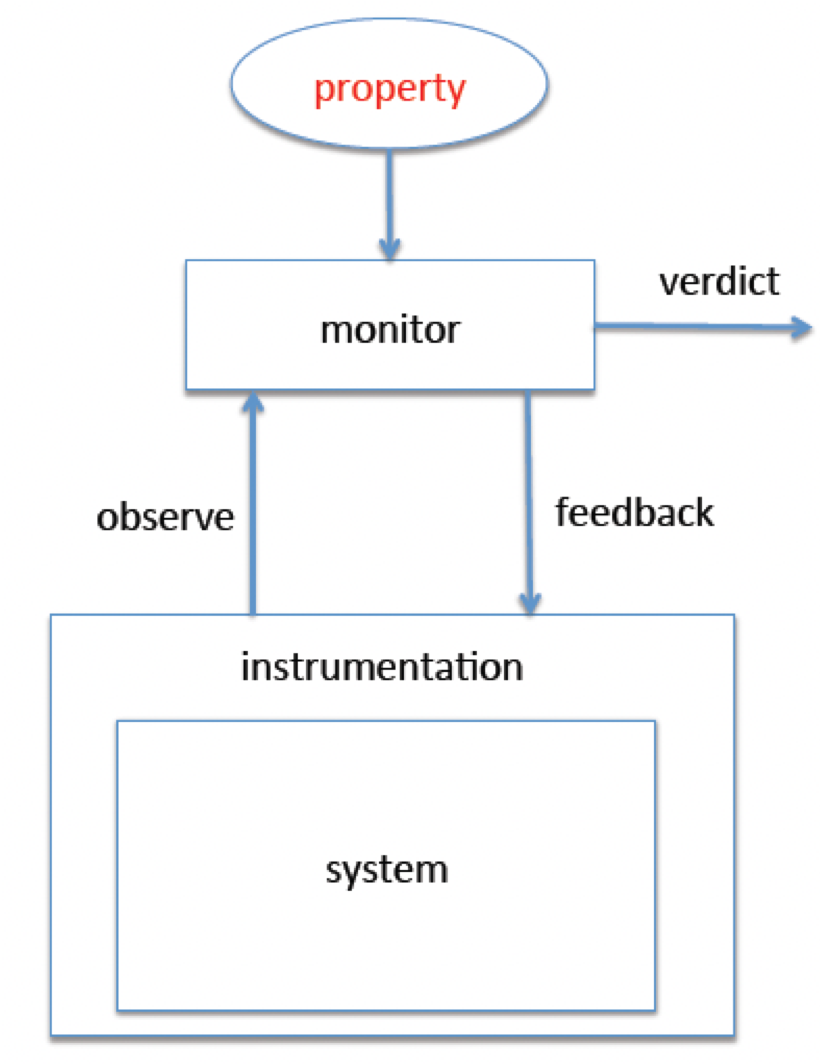
\includegraphics [scale=0.4]{Images/rv.png}
    \caption{An overview of the RV process}
    \label{rv}
\end{figure}

 The components of a RV environment are the system to be checked and a set of properties to be checked against the system execution. Properties can be expressed in a formal specification language, or even as a program in a general-purpose programming language. From a given property, a monitor is generated, i.e., a decision procedure for that property - \textit{monitor synthesis}. The system is instrumented to generate the relevant events to be fed into the monitor - \textit{system instrumentation}. In the next step, the system's execution is analyzed by the monitor - \textit{execution analysis}. The monitor is able to consume the events produced by the running system and, for each consumed event, emits a verdict indicating the status of the property, depending on the event sequence seen so far. Finally, the monitor sends feedback to the system so that more specific corrective actions can be taken (Figure \ref{rv}) ~\cite{rvart}.
 
 
\subsection{Formal Specification of the system behaviour}
There are different formal approaches to describe the expected behaviour of a system. But before presenting some different specification languages, let's start by presenting some general properties of these formalisms. 

\subsubsection{Events}
The behaviour of a system can be analyzed as the way the system changes over time, and this can be done through its observation. To abstract these observations we will use \textit{Events} - discrete atomic entities that represent \textit{actions} or \textit{state changes} made by the system. 
The system's observable events of interest is called its \textit{alphabet}. The choice of events is part of the specification and will determine the available information about the system and about which properties can be described.

\subsubsection{Traces}
A \textit{trace} is a sequence of events and abstracts the behaviour of a single run of the system. Obviously, an observable trace must be finite, but it is sometimes useful to think about the possible infinite behaviours of a system. Therefore, a trace can be viewed as a finite prefix of the infinite behaviour.

\subsubsection{Properties and Specifications}
The abstraction of a property can be described as a set of traces and its specification is a concrete (textual) object that denotes this set of traces.
As there are many specifications languages, one can have many specifications for a single property, but a property is unique and independent of the specification language. If the specification language is ambiguous, then the specific property may not be clear. Dealing with such ambiguities is a common issue in the specification process ~\cite{rv2}.


\subsection{Different language specifications}
This section presents a brief description of the main specification languages for RV, as well as some of their general features.

A RV specification language can be \textit{Executable} if the specification is directly executable and therefore more low-level, or \textit{Declarative} in which an executable object (monitor) is generated from the specification. Also, some specification languages are more suited to specify sets of finite traces whereas others are more suited to specify infinite traces. A specification may also capture \textit{good} or \textit{bad} behaviour. A match against a good behaviour specification represents \textit{validation} of the desired property, whereas a match a bad behaviour specification represents \textit{violation} of that property ~\cite{rv2}.

\subsubsection{Regular Expressions}
Regular Expressions are a commonly used formalism in Computer Science for describing sets of strings, but can also be used in RV to describe traces of events, where the atoms are not characters but events. The regular expression matches if any \textit{suffix} of the trace matches the expression - \textit{suffix-matching} - to attest the validation or violation of the property (e.g., in the work of TraceMatches) ~\cite{rvart}.

\subsubsection{Finite State Machines}
Finite State machines have the same expressive power of Regular Expressions but have the advantage of being directly executable, in opposition to regular expressions and temporal logic, since both require \textit{monitor synthesis} to produce a monitor, which is usually described as some form of state machine. 

\vspace{5mm}

The formalisms of \textbf{Linear Temporal Logic} and \textbf{Context Free Grammars} can also be used for specifications in RV, but since they are not the main focus of the present work they will not be further approached. 

    
    \section{Bidirectional Transformations}

Bidirectional Transformations (BX) provide a mechanism for maintaining consistency between two pieces of data. A bidirectional transformation consists of a pair of functions: a \textit{get} function that extracts part of information from a source to produce a view, and a \textit{put} function that accepts an updated view and the original source, producing an updated source that is consistent with the new view. The pair of functions needs to satisfy the \textit{well-behavedness} laws:

\begin{flalign*}
    put\ s\ (get\ s) = s \quad (GetPut) \\
    get\ (put\ s\ v)\ = v \quad (PutGet)
\end{flalign*}

The \textit{GetPut} law says that \textit{put} an unmodified view \textit{get s} into the source should produce the same unmodified source $s$. The \textit{PutGet} law says that getting from an updated source computed by \textit{put}ting a view $v$ should retrieve the same $v$. 
	
    \section{Regular Expressions and Finite State Machine}

Regular expressions and Finite Automata (FA) represent a valuable concept in theoretical computer science. Their equivalence is well known dating back to the Kleen's paper in 1956. REs are well suited for human users and therefore often used as interfaces to specify certain patterns or languages, while automata immediately translate to efficient data structures and are suited for programming tasks. Obviously this fact raises the interest in conversion algorithms between them ~\cite{refa}. 

Moreover, when reasoning about the specifications of properties for RV, it can be useful to convert between them and observe how changes in one of the specifications are reflected in the other. That was the main motivation for use Bidirectional Transformations between these two types of specifications.

The next sections will describe some formal definitions of RE and FA as well as the known algorithms to convert between them. 

\subsection{Formal definitions}
\label{definitions}
Before introduce the known algorithms for conversion it is useful to present and formally describe the two types of automata. 

\subsubsection{Regular Expressions} 
Given a vocabulary $\Sigma$, a symbol $a \in \Sigma$ and the regular expressions $s$ and $t$, then RE can be defined inductively as following: 

\begin{equation*}
    RE = \quad \emptyset \quad | \quad \epsilon \quad | \quad a \quad | \quad (s+t) \quad | \quad (s\ .\ t) \quad | \quad (s)^*
\end{equation*}

The language defined by a regular expression $r$, denoted by $L(r)$, is defined as follows:

\begin{flalign*}
    L(\emptyset) & = \emptyset \\
    L(\epsilon) & = \{\epsilon\} \\
    L(a) & = \{a\} \\
    L(s+t) & = L(s) \cup L(t) \\
    L(s\ .\ t) & = L(s)\ .\ L(t) \\
    L(s^*) & = L(s)^*
\end{flalign*}

\subsubsection{Non-Deterministic Finite Automata (NDFA)} Formally, a NDFA is described as follows:  

\begin{equation*}
    A = (Q,\Sigma,q_0,F,\delta)
\end{equation*}

where, $Q$ is the finite set of states, $\Sigma$ is the finite set of input symbols (the vocabulary), $q_0 \in Q$ is the initial states, $F \in Q$ is the set of accepting (final) states, and $\delta : Q \times (\Sigma \cup \{\epsilon\}) \rightarrow 2^Q$ is the \textit{transition function}. 

As the name itself pronounces, the NDFA can transit to one or more states when consuming a given symbol. The next state is computed as the set of all possible states to which is possible to transit. The NDFA can have \textit{$\epsilon$-transitions}, transitions without consuming any input symbol, i.e. the empty string $\epsilon$ is a possible input. 
If the NDFA has no $\epsilon$-transitions, i.e. is $\epsilon$-free, then the transition function can be restricted to $\delta : Q \times \Sigma \rightarrow 2^Q$.

\subsubsection{Deterministic Finite Automata (DFA)} \textit{Deterministic} refers to the uniqueness of the computation. It can be seen as a special kind of NDFA in which for each state and symbol, the result of the transition has exactly one state. Following is the formal definition of a DFA:

\begin{equation*}
    A = (Q,\Sigma,q_0,F,\delta)
\end{equation*}

where, $Q$ is the finite set of states, $\Sigma$ is the finite set of input symbols (the vocabulary), $q_0 \in Q$ is the initial state, $F \in Q$ is the set of accepting (final) states, and $\delta : Q \times \Sigma \rightarrow Q$ is the \textit{transition function}. 

\subsection{Conversion algorithms}
This sections recalls the most prominent algorithms for conversion from a RE to a DFA. 

\subsubsection{Thompson's construction algorithm}
Converts a RE into an equivalent NDFA. The algorithm splits an expression into its constituent sub-expressions and works recursively applying the next rules: 

\begin{itemize}
    \item  $\bf e = \emptyset$ is converted in:
    \begin{figure}[H]
        \begin{center}
        \resizebox{.3\textwidth}{!}{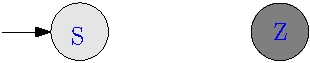
\includegraphics{Images/NdfaREempty.pdf}}
        \end{center} 
    \end{figure}
    
    \item $\bf e = \epsilon$  is converted in:
    \begin{figure}[H]
        \begin{center}
        \resizebox{.1\textwidth}{!}{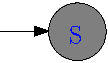
\includegraphics{Images/NdfaREepsilon.pdf}}
        \end{center} 
    \end{figure}
    
    \item  $\bf e = a$ is converted in:
    \begin{figure}[H]
        \begin{center}
        \resizebox{.3\textwidth}{!}{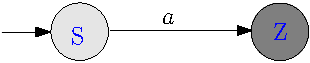
\includegraphics{Images/NdfaRElit.pdf}}
        \end{center} 
    \end{figure}
    
    \item  $\bf e = p\ .\ q$ is converted in:
    \begin{figure}[H]
        \begin{center}
        \resizebox{.7\textwidth}{!}{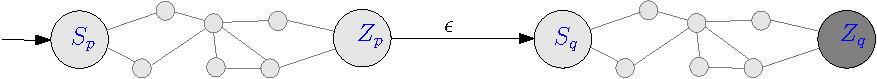
\includegraphics{Images/NdfaREthen.pdf}}
        \end{center} 
    \end{figure}
    
    \item  $\bf e = p + q$ is converted in:
    \begin{figure}[H]
        \begin{center}
        \resizebox{.6\textwidth}{!}{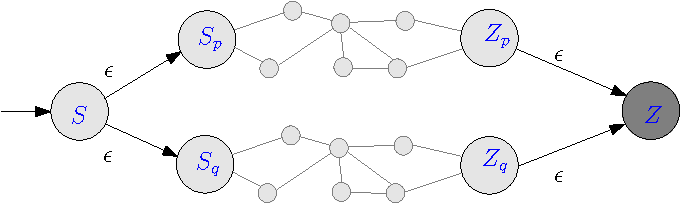
\includegraphics{Images/NdfaREor.pdf}}
        \end{center} 
    \end{figure}
    
    \item  $\bf e = p^*$ is converted in:
    \begin{figure}[H]
        \begin{center}
        \resizebox{.6\textwidth}{!}{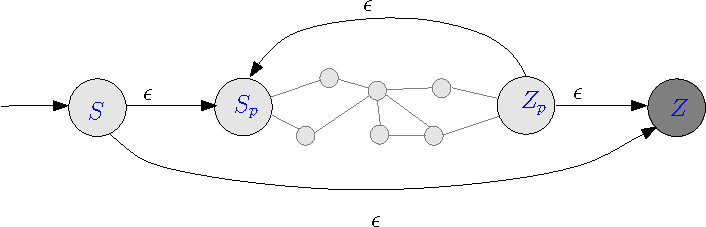
\includegraphics{Images/NdfaREstar.pdf}}
        \end{center} 
    \end{figure}
\end{itemize}

For instance, the regular expression $\bf e = (\epsilon + a^*b)$ would be converted in the NDFA presented in Figure \ref{fig:ndfaT}

\begin{figure}
    \centering
    \resizebox{.8\textwidth}{!}{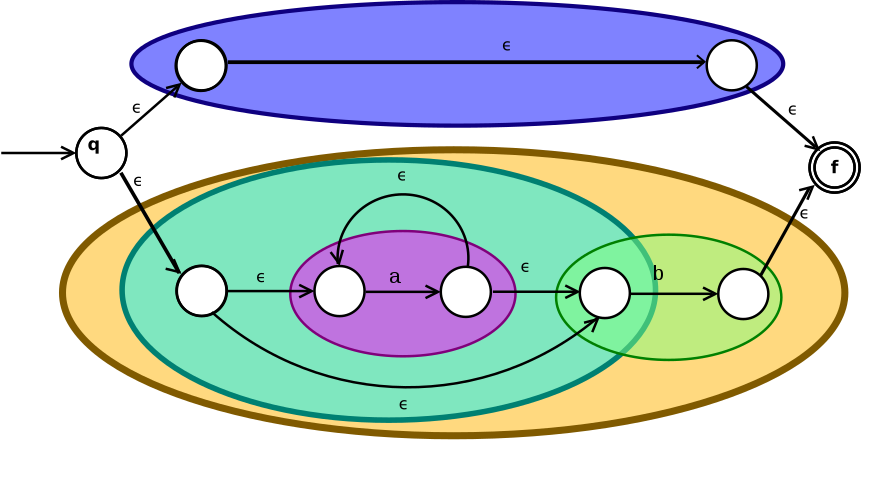
\includegraphics{Images/ndfa.png}}
    \caption{NDFA resulting from $\bf e = (\epsilon + a^*b)$ using Thompson's construction }
    \label{fig:ndfaT}
\end{figure}


\subsubsection{Glushkov's construction algorithm}
Is another well-known algorithm to convert a give RE into a NDFA. Is similar to Thompson's construction, once the $\epsilon$-transitions are removed. Following are the construction steps to create a NDFA that accepts the language $L(e)$ accepted by the RE $e$:

\begin{itemize}
    \item \textbf{Step 1} - linearisation of the expression. Each letter of the alphabet appearing in the expression e is renamed, so that each letter occurs at most once in the new expression $e'$. Let $A$ be the old alphabet and let $B$ be the new one;
    \item \textbf{Step 2a} - the following sets are computed:
    \begin{itemize}
        \item $P(e') = \{\ x \in B\quad |\quad xB^* \cap L(e') \neq \emptyset\ \}$  is the set of symbols which occurs as first letter of a word of $L(e')$. Can be defined inductively:
        
        \begin{flalign*}
            P(\emptyset) & = P(\epsilon) = \emptyset \\
            P(a) & = \{a\} \text{, for each letter $a$} \\
            P(s+t) & = P(s) \cup P(t) \\
            P(s\ .\ t) & = P(s)\ \cup \ \Lambda (s) P(t) \\
            P(s^*) & = P(s)
        \end{flalign*}
        
        
        \item $D(e') = \{\ y \in B\quad |\quad B^*y \cap L(e') \neq \emptyset\ \}$ is the set of symbols that can end a word of $L(e')$. Can be defined inductively with the same rules of $P$ except for the product where
        
        \begin{equation*}
            D(s\ .\ t) = D(t)\ \cup \ D(s)\Lambda(t) 
        \end{equation*}
        
        \item $F(e') = \{\ u \in B^2\quad |\quad B^*uB^* \cap L(e') \neq \emptyset\ \}$ is the set f symbol pair that can occur in words of $L(e')$. Can be defined inductively as follows: 
        \begin{flalign*}
            F(\emptyset) & = F(\epsilon) = F(a) = \emptyset \text{, for each letter $a$} \\
            F(s+t) & = F(s) \cup F(t) \\
            F(s\ .\ t) & = F(s)\ \cup\ F(t)\ \cup\ D(s)P(t) \\
            F(s^*) & = F(s)\ \cup\ D(e)P(e)
        \end{flalign*}
        
    \end{itemize}
    
    \item \textbf{Step 2b} - computes the set $\Lambda = \{\epsilon\} \cup L(e')$, in case the empty word belongs to the language, otherwise $\Lambda = \emptyset$. It can be defined inductively for each RE as following:
    \begin{flalign*}
        \Lambda(\emptyset) & = \emptyset \\
        \Lambda(\epsilon) & = \{\epsilon\} \\
        \Lambda(a) & = \emptyset \text{, for each letter $a$} \\
        \Lambda(s+t) & = \Lambda(s) \cup \Lambda(t) \\
        \Lambda(s\ .\ t) & = \Lambda(s)\ .\ \Lambda(t) \\
        \Lambda(s^*) & = \{\epsilon\} 
    \end{flalign*}
    
    
    \item \textbf{Step 3} - computation of the local language, i.e. the set of words which begin with a letter of $P$, end by a letter of $D$ and whose transitions belong to $F$: 
    \begin{equation*}
        L' = (PB^* \cap B^*D)\ \backslash\ B^* (B^2 \backslash F) B^*
    \end{equation*}
    
    \item \textbf{Step 4} - erasing the delinearization, giving to each letter of $B$ the letter of $A$.
\end{itemize}

Given the regular expression $\bf e = (a(ab)^*)^* + (ba)^*$, would produce the NDFA in Figure \ref{fig:ndfaG}, without performing Step 4, to perform this step one only needs to remove the index from each symbol in the nodes.

\begin{figure}
    \centering
    \resizebox{.8\textwidth}{!}{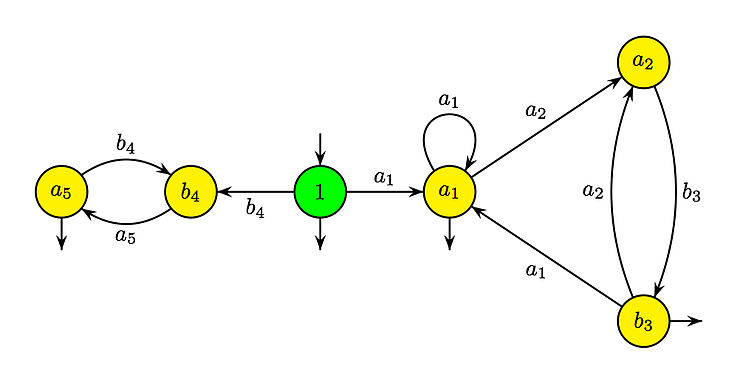
\includegraphics{Images/glushkov.jpg}}
    \caption{NDFA resulting from $\bf e = (a(ab)^*)^* + (ba)^*$ using Glushkov's construction }
    \label{fig:ndfaG}
\end{figure}

\subsubsection{Powerset construction algorithm}
Converts a NDFA into a DFA, which recognize the same formal language. Recall the structure of a NDFA in Section \ref{definitions}, the corresponding DFA has the set of states $Q_D$, where each state corresponds to subsets of $Q_N$. 

The initial state of the DFA is the set $\{q_0\}$ where $q_0$ is the initial state of the NDFA. In case of a NDFA has $\epsilon$-transitions then the initial state of the DFA - $q_{0D}$ - has the initial state of the NDFA - $q_{0N}$ - plus the states reachable from that state through $\epsilon$-transitions - called $\epsilon$-\textit{closure}:
\begin{equation*}
    q_{0D} = q_{0N}\ \cup \ \epsilon\text{-\textit{closure}} \ \{q_{0N}\}
\end{equation*}

Starting from the initial state $q_{0D}$, each new state is computed from another state $S \in Q_D$. It can be defined recursively as:
\begin{itemize}
    \item $q_{0D} \in Q_D$
    \item $qs \in Q_D \Rightarrow \{ d\ |\ (o,y,d) \in \delta_{NDFA} \wedge o \in qs\} \in Q_Dv , \quad \forall y \in \Sigma$
\end{itemize}

The transition function of the DFA maps a state $S$ and the input symbol $y$ to the respective computed state:

\begin{equation*}
    \delta_{DFA} = \cup \{(S,y,D) | D = \{ d\ |\ (o,y,d) \in \delta_{NDFA} \wedge o \in S\}\}, \forall{(y \in \Sigma \wedge S \in Q_D)}
\end{equation*}

Finally, the set of accepting states of the DFA $Z_D$ is the set of states $S \in Q_D$ that contain at least one state that is accepting state in the NDFA:

\begin{equation*}
    Z_D = \{q \in Q_D\ |\ q \cap Z_N \neq \emptyset\}
\end{equation*}

\subsubsection{Kleene's Algorithm}

Kleene's algorithm produces a regular expression from a DFA in the following way.
\begin{enumerate}
    \item It first constructs a graph whose nodes correspond to the states of the automaton and the edges are regular expressions that connect those nodes. 
    \item The initial set of edges contains one edge for each transition in the automaton (labelled with the corresponding literal) plus one edge for each node to itself containing the regular expression $\epsilon$.
    \item It proceeds by applying a variation of the Floyd-Warshall algorithm in order to obtain all paths connecting each of the nodes (summing weights corresponds to concatenation of regular expressions whereas the minimum operation corresponds to alternative ($+$) of regular expressions).
    \item Finally the regular expression equivalent to the original DFA can be obtained as the union ($+$) of the edges which connect the initial state to all final states.
\end{enumerate}
	
    \section{Implementation}
This section describes the process of implementing BX between a RE and a DFA. It will start by describing the reasoning about how to implement the BX and will follow by explaining the implementation process, including the explanation about the algorithm's choices. Finally, it will present the \textit{put} strategy defined for a BX between NDFA and DFA.

The source code of the implementation is available in the Github repository:  \url{https://github.com/lisandrasilva/rv-bx}.

\subsection{Reasoning about BX}
Considering the already existent algorithms to convert between a RE and a DFA, we decided to attempt implementing the BX as a composition of two small BX, more concretely, one between RE and NDFA and another between NDFA and DFA. As depicted in Figure \ref{fig:BX} the NDFA would be an intermediate structure used as a view in one of the BX and as a source in the another.  

\begin{figure}
    \centering
    \resizebox{.4\textwidth}{!}{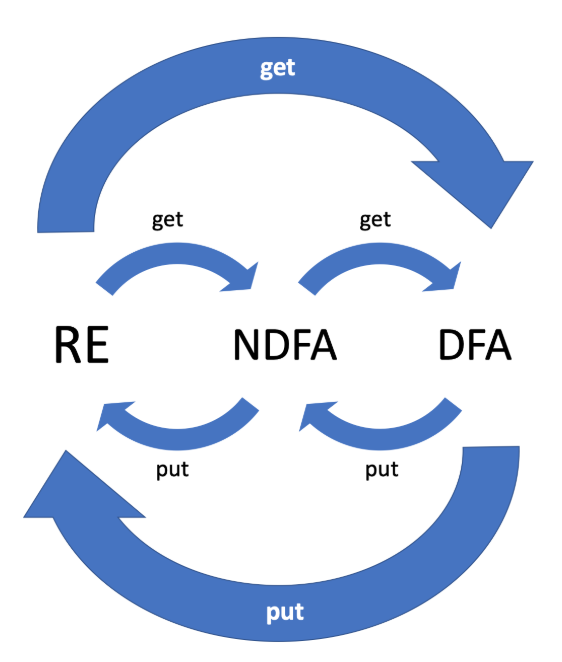
\includegraphics{Images/BX_arc.png}}
    \caption{BX between RE and DFA}
    \label{fig:BX}
\end{figure}

In the BX between RE and NDFA the source is the RE and the view is the NDFA. The \textit{getNDFA} function from RE to NDFA would be one of the conversion algorithms presented on Section \ref{convert} - Thompson's construction or Glushkov's construction. Regarding the BX between NDFA and the DFA, the source is the NDFA and the view is the DFA, where the \textit{getDFA} function would be the Powerset construction algorithm.

\vspace{5mm}
The \textit{get} function that given a RE as source and produces a DFA as view will be the composition of these two functions:

\begin{center}
    \textit{\textbf{get re} = (getDFA . getNDFA) re}
\end{center}

\vspace{5mm}
The main goal is to define the \textit{putback} functions:

\vspace{3mm}
\textbf{\textit{putNDFA}} - function that accepts a NDFA as a source and a possible modified DFA as a view and reflects the changes on the view into the source;
    
\textbf{\textit{putRE}} - function that accepts a RE as a source and a possible modified NDFA as a view and reflects the changes on the view into the source.

\vspace{5mm}
The final \textit{putback} function that accepts a RE as a source and a possible modified DFA as a view and produces the updated RE will be the composition of these two functions:


\begin{center}
    \textit{\textbf{put re dfa} = putRE re (putNDFA (get re) dfa)}
\end{center}

To tackle the problem we decided to start by define the \textit{putNDFA} function.

\subsection{Get function}
As said above the \textit{get} function will be the composition of two, with a NDFA as an intermediate structure. Once this NDFA will be the source argument of the \textit{putNDFA} function and the view argument for the \textit{putRE} function, it is necessary to reason about what type of NDFA we should consider, which means reason about the choice for the \textit{getNDFA} function.

The NDFA can be obtained through the Thompson's construction algorithm or through the Glushkov's construction algorithm. But, recall that the resulting NDFA are different since the one obtained through Glushkov's algorithm is \textit{$\epsilon$-free}, while the one obtained through the Thompson's algorithm has $\epsilon$-transitions. 

\subsubsection{NDFA with $\epsilon$-transitions}
Let's consider the NDFA in Figure \ref{fig:epsilon} and its correspondent DFA in Figure \ref{fig:epsilondfa} obtained through the Powerset construction algorithm. 

\begin{figure}
    \centering
    \resizebox{.7\textwidth}{!}{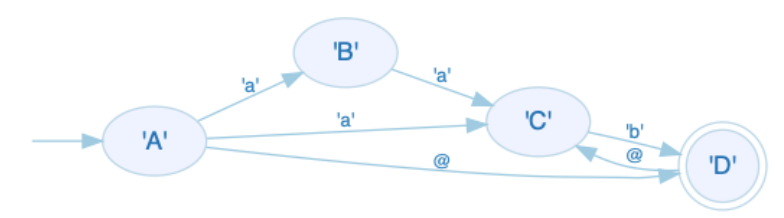
\includegraphics{Images/epsilondfa.png}}
    \caption{NDFA with $\epsilon$-transitions}
    \label{fig:epsilon}
\end{figure}

\begin{figure}
    \centering
    \resizebox{.7\textwidth}{!}{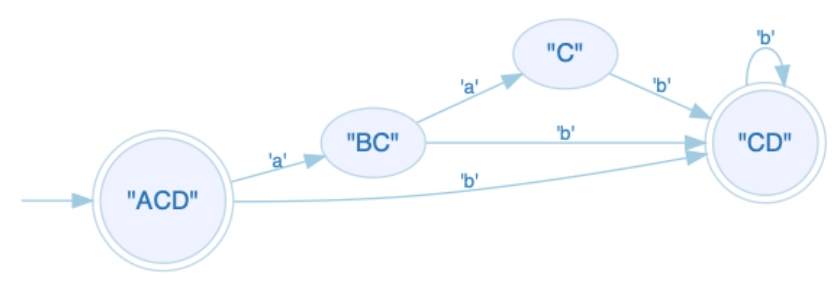
\includegraphics{Images/epsilon_DFA.png}}
    \caption{DFA obtained from NDFA in Figure \ref{fig:epsilon}}
    \label{fig:epsilondfa}
\end{figure}

By analyzing  those figures is becomes clear that it is hard to reason about a \textit{putback} function when the NDFA has $\epsilon$-transitions. For instance, in the obtained DFA of the given example (Figure \ref{fig:epsilondfa}) all the nodes are dependent on the transitions of the 'C' node in the NDFA, which means that when adding or removing transitions from or to node 'C' in the NDFA, these changes will be reflected in all the nodes with 'C' in the DFA (because that is what is demanded by the Powerset construction).

This fact restricts too much the possible changes in the view, and even though we designed a pseudo-algorithm to \textit{put} function in many cases it didn't satisfied the GetPut law. 

\subsubsection{NDFA \textit{$\epsilon$-free}} Figure \ref{fig:glundfa} depicts a \textit{$\epsilon$-free} NDFA equivalent to the NDFA in Figure \ref{fig:epsilondfa} and in Figure \ref{fig:gludfa} its the correspondent DFA. 

\begin{figure}[H]
    \centering
    \resizebox{.8\textwidth}{!}{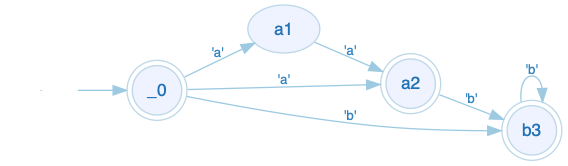
\includegraphics{Images/Glushkovdot.png}}
    \caption{NDFA \textit{$\epsilon$-free}}
    \label{fig:glundfa}
\end{figure}

\begin{figure}
    \centering
    \resizebox{.8\textwidth}{!}{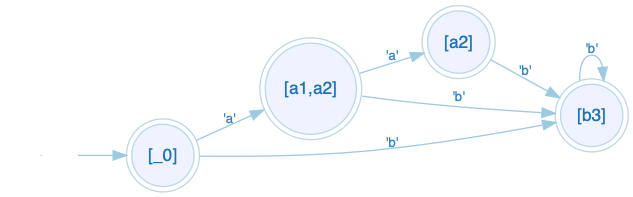
\includegraphics{Images/gluDFAdot.png}}
    \caption{DFA obtained from NDFA in Figure \ref{fig:epsilon}}
    \label{fig:gludfa}
\end{figure}

By analyzing the two automata, we can conclude that there are less dependencies, the only dependency is between nodes \texttt{[a1,a2]} and \texttt{[a2]}, because both have the node \texttt{a2} from the NDFA. Therefore changes in this node will be reflected in both nodes in the view, even when only one was modified in the first place. 

However, as it allows a wider range of possible changes on the view, we decided to choose the \textit{$\epsilon$-free} NDFA to define the \textit{put} strategy between NDFA and DFA, meaning that the \textit{get} function from RE to NDFA should be the Glushkov's construction algorithm. 

\subsection{Put back from DFA to NDFA}

\subsubsection{Structures for DFA and NDFA}
When reasoning about the put back function, the first step was to define the structures to represent both the NDFA and the DFA. Both structures are structurally very similar, but they will differ in the transition table \texttt{delta}, since in the DFA is not allowed to have two transitions from the same node with the same symbol, while in the NDFA that is possible. 

\begin{verbatim}
data Ndfa st sy = Ndfa { vocabularyN :: [sy ],
                         statesN     :: [st ],
                         initialSN   :: [st ],
                         finalSN     :: [st ],
                         deltaN      :: [((st,sy),st)]
                       }
                   
data Dfa st sy = Dfa { vocabularyD :: [sy],
                       statesD     :: [st],
                       initialSD   :: st,
                       finalSD     :: [st],
                       deltaD      :: [((st,sy),st)]
                     }
\end{verbatim}

We decided to represent the structures with polymorphism on the arguments so they can be more flexible on the types they can represent. However, remind that in the present work, the DFA is result of the Powerset construction of the NDFA, which means that the states in the DFA are sets of the states in the NDFA. As so, if in NDFA the type of \texttt{st} is for example \texttt{Int}, then the type of \texttt{st} in the DFA is \texttt{[Int]}. 

Table \ref{tablestruct} shows how the automata in Figures \ref{fig:glundfa} and \ref{fig:gludfa} are (pretty-printed) represented in the data structures mentioned above.

\begin{table}
  \begin{center}
    \begin{tabular}{ | p{3cm} |p{4cm}||p{4cm}|  }
    \hline
         & NDFA & DFA \\ [1ex]
        \hline
        \hline
        Vocabulary & `b', `a' & `b', `a'\\ [0.7ex]
        \hline
        States & \_0, b3, a2, a1 & [a2], [a1,a2], [b3], [\_0]\\ [0.7ex]
        \hline
        Initial State & \_0 & [\_0] \\ [0.7ex]
        \hline
        Final States & \_0, a2, b3 & [a2], [a1,a2], [b3], [\_0] \\ [0.7ex]
        \hline
        \multirow{3}{5em}{Transition Table} & \_0 $\xrightarrow{'a'}$ a1 & [\_0] $\xrightarrow{'a'}$ [a1,a2]\\
        & \_0 $\xrightarrow{'b'}$ a2 & [\_0]    $\xrightarrow{'b'}$ [b3]\\
        & \_0 $\xrightarrow{'b'}$ b3 & [a1,a2]  $\xrightarrow{'a'}$ [a2]\\
        & a1  $\xrightarrow{'b'}$ a2 & [a1,a2]  $\xrightarrow{'b'}$ [b3]\\
        & a2  $\xrightarrow{'b'}$ b3 & [a2]     $\xrightarrow{'b'}$ [b3]\\
        & b3  $\xrightarrow{'b'}$ b3 & [b3]     $\xrightarrow{'b'}$ [b3]\\
        \hline
        \end{tabular}
  \end{center}
  \caption{Representation of automata in Figures \ref{fig:glundfa} and \ref{fig:gludfa}}
  \label{tablestruct}
\end{table}

\subsubsection{Reflecting transition table}
The function \texttt{getTable} is responsible for reflecting the DFA transition table into the NDFA transition table. Therefore, it receives as argument the NDFA transition table, the DFA transition table and the set of states $q$ of the DFA (to perform checks) and returns the updated NDFA transition table. The argument with the DFA transition table is in fact zipped with an accumulator that will save, for each DFA transition $os \xrightarrow{s} ds$, the subset of $ds$ of the NDFA transitions that were validated so far. 

The code presented below can be better understood with the example given afterwards. 

\begin{verbatim}
getTable :: (Ord st, Ord sy) =>[((st,sy),st)] 
                             ->[((([st],sy),[st]),[st)]
                             -> [[st]] 
                             ->[((st,sy),st)]
getTable [] dfaT q = 
    let toAdd = filter (not . null . snd)
                [(((os,d),ds\\rs)) |(((os,d),ds),rs) <- dfaT]
    in concat $ map (`rearrangeS' q)toAdd
    
getTable (t@((o,s),d):ts) dfaT q = 
    let relS = [ x | x <- q , o `elem' x]
        trns = [ 1 | (((os,sym),ds),rs) <- dfaT , 
                                           os `elem' relS ,
                                           sym == s , 
                                           d `elem' ds]
        dfaT' = map (updateListAux t) dfaT
    in if (length relS == length trns) && (not $ null relS) 
       then t:getTable ts dfaT' q
       else getTable ts dfaT q
\end{verbatim}

\vspace{5mm}
%The function consumes each NDFA transition table recursively. 
For each NDFA transition \texttt{((o,s),d)}, the function verifies that each node in the DFA that contains `$o$' has the transition through symbol `$s$' for a node that contains `$d$'. When this is valid then the NDFA transition is kept in the source and the `$d$' is added to the auxiliary list from the DFA transitions mentioned above (using \texttt{updateListAux} function), otherwise is discarded. 



\begin{verbatim}
updateListAux ((o,s1),d)(((os,s2),ds),rs) = 
            if o `elem' os && s1 == s2 &&d `elem' ds
            then (((os,s2),ds),d:rs)
            else (((os,s2),ds),rs)
\end{verbatim}

Going back to the example in Figures \ref{fig:glundfa} and \ref{fig:gludfa}, let's do the following sequence of modifications on the view (depicted in DFA in Figure \ref{fig:updatedfa}):

\begin{itemize}
    \item Remove transition [a2] $\xrightarrow{'b'}$ [b3]
    \item Add transition [a1,a2] $\xrightarrow{'c'}$ [c4]
    \item Add transition [c4] $\xrightarrow{'b'}$ [b3]
\end{itemize}


\begin{figure}
    \centering
    \resizebox{.85\textwidth}{!}{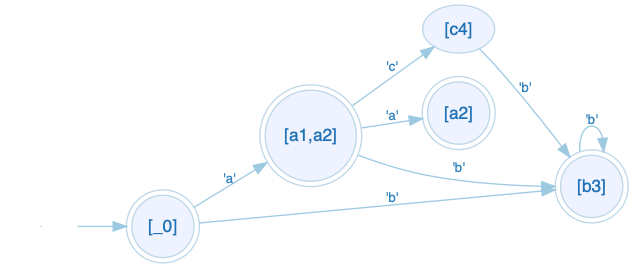
\includegraphics{Images/updatedDFA.png}}
    \caption{Updated view}
    \label{fig:updatedfa}
\end{figure}

Table \ref{getTable} represents the arguments to the function \texttt{getTable} with the updated DFA transition table.
As mentioned, the function \texttt{getTable} goes recursively through the NDFA transitions. For the first NDFA transition \texttt{((\_0,'a'),a1)} the function gets all the DFA states that contain \_0 (which is only [\_0]), and ensures that it has the transition through 'a' to a node which contains a1. As this is true due to the transition \texttt{(([\_0],'a'),[a1,a2])} then a1 is added to the auxiliary accumulator list of the transition.

\begin{table}[H]
  \begin{center}
    \begin{tabular}{ | p{3cm} |p{4cm}||p{3cm} p{1cm} |  }
    \hline
         & NDFA & DFA & \\ [1ex]
        \hline
        States & \_0, b3, a2, a1 & [a2], [a1,a2], [b3], [\_0], & [c4] \\ [0.7ex]
        \hline
        \multirow{3}{5em}{Transition Table} & \_0 $\xrightarrow{'a'}$ a1 & [\_0] $\xrightarrow{'a'}$ [a1,a2] & [ ]\\
        & \_0 $\xrightarrow{'b'}$ a2 & [\_0]    $\xrightarrow{'b'}$ [b3] & [ ]\\
        & \_0 $\xrightarrow{'b'}$ b3 & [a1,a2]  $\xrightarrow{'a'}$ [a2] & [ ]\\
        & a1  $\xrightarrow{'b'}$ a2 & [a1,a2]  $\xrightarrow{'b'}$ [b3] & [ ]\\
        & a2  $\xrightarrow{'b'}$ b3 & \textcolor{gray}{[a2]     $\xrightarrow{'b'}$ [b3]} &  \\
        & b3  $\xrightarrow{'b'}$ b3 & [b3]     $\xrightarrow{'b'}$ [b3] & [ ]\\
        &  & \textcolor{ForestGreen}{[a1,a2]  $\xrightarrow{'c'}$ [c4]} & \textcolor{ForestGreen}{[ ]}\\
        &  & \textcolor{ForestGreen}{[c4]  $\xrightarrow{'b'}$ [b3]} & \textcolor{ForestGreen}{[ ]}\\
        \hline
        \end{tabular}
  \end{center}
  \caption{Arguments for \texttt{getTable} with updated view}
  \label{getTable}
\end{table}

When analyzing NDFA transition \texttt{((a2,'b'),b3)}, all the DFA nodes that contain \texttt{a2} (\texttt{[a1,a2]} and \texttt{[a2]}) must have the transition through \texttt{'b'} to a node that contains \texttt{b3}. However this is not verified since the DFA transition \texttt{(([a2],'b'),[b3])} was removed from the view, therefore this NDFA transition is not kept in the source.


\begin{table}[H]
  \begin{center}
    \begin{tabular}{ | p{3cm} |p{4cm}||p{3cm} p{1cm} |  }
    \hline
         & NDFA & DFA & \\ [1ex]
        \hline
        States & \_0, b3, a2, a1 & [a2], [a1,a2], [b3], [\_0], & [c4]\\ [0.7ex]
        \hline
        \multirow{3}{5em}{Transition Table} & \textcolor{blue}{\_0 $\xrightarrow{'a'}$ a1} & [\_0] $\xrightarrow{'a'}$ [a1,a2] & [\textcolor{blue}{a1,a2}]\\
        & \textcolor{blue}{\_0 $\xrightarrow{'b'}$ a2} & [\_0]   $\xrightarrow{'b'}$ [b3] & [\textcolor{blue}{b3}]\\
        & \textcolor{blue}{\_0 $\xrightarrow{'b'}$ b3} & [a1,a2]  $\xrightarrow{'a'}$ [a2] & [\textcolor{blue}{a2}]\\
        & \textcolor{blue}{a1  $\xrightarrow{'b'}$ a2} & [a1,a2]  $\xrightarrow{'b'}$ [b3] & [ ]\\
        & \textcolor{gray}{a2  $\xrightarrow{'b'}$ b3} & \textcolor{gray}{[a2]     $\xrightarrow{'b'}$ [b3]} &  \\
        & \textcolor{blue}{b3  $\xrightarrow{'b'}$ b3} & [b3]     $\xrightarrow{'b'}$ [b3] & [\textcolor{blue}{b3}]\\
        &  & \textcolor{ForestGreen}{[a1,a2]  $\xrightarrow{'c'}$ [c4]} & \textcolor{ForestGreen}{[ ]}\\
        &  & \textcolor{ForestGreen}{[c4]  $\xrightarrow{'b'}$ [b3]} & \textcolor{ForestGreen}{[ ]}\\
        \hline
        \end{tabular}
  \end{center}
  \caption{Transition tables after \texttt{getTable} processed all old NDFA transitions}
  \label{getTable2}
\end{table}

Table \ref{getTable2} contains the state of the transition tables after the function \texttt{getTable} already processed all the NDFA transitions. After that, the function \texttt{getTable} is recursively called with the first argument (NDFA table transtion) empty. At this point, for each DFA transition \texttt{((os,s),ds)} its corresponding auxiliary list with the subset of $ds$ that were already validated is removed from the set $ds$. If the remaining $ds$ list is empty then it means that the transition was already validated. When there are still states in the list $ds$, the new transitions in the NDFA must be created (Table \ref{getTable3}). This is done in the \texttt{rearrangeS} function. 

\begin{table}
  \begin{center}
    \begin{tabular}{ | p{3cm} |p{4cm}||p{3cm} p{1cm} |  }
    \hline
         & NDFA & DFA & \\ [1ex]
        \hline
        States & \_0, b3, a2, a1 & [a2], [a1,a2], [b3], [\_0], & [c4]\\ [0.7ex]
        \hline
        \multirow{3}{5em}{Transition Table} & \textcolor{blue}{\_0 $\xrightarrow{'a'}$ a1} & [a1,a2]  $\xrightarrow{'b'}$ [b3] & [ ]\\
        & \textcolor{blue}{\_0 $\xrightarrow{'b'}$ a2} & \textcolor{ForestGreen}{[a1,a2]  $\xrightarrow{'c'}$ [c4]} & \textcolor{ForestGreen}{[ ]}\\
        & \textcolor{blue}{\_0 $\xrightarrow{'b'}$ b3} & \textcolor{ForestGreen}{[c4]  $\xrightarrow{'b'}$ [b3]} & \textcolor{ForestGreen}{[ ]}\\
        & \textcolor{blue}{a1  $\xrightarrow{'b'}$ a2} & & \\
        & \textcolor{blue}{b3  $\xrightarrow{'b'}$ b3} & & \\
        \hline
        \end{tabular}
  \end{center}
  \caption{Transition tables before call \texttt{rearrangeS} function}
  \label{getTable3}
\end{table}

The function receives a DFA transition, the set of DFA states and creates the list of new NDFA transitions corresponding to the given DFA transition. 
First the function computes the minimum list of NDFA transitions, excluding transitions whose origin appears in other DFA nodes. 

\begin{verbatim}
rearrangeS :: Eq st => (([st], sy), [st])
                    -> [[st]] 
                    -> [((st, sy), st)]
rearrangeS ((os,sy),dsts) q = 
    let min = [((o,sy),dd) | o <- os \\ (concat $ delete os q), 
                             dd <- dsts]
    in if null min then [((o,sy),dd) | o <- os, dd <- dsts]
       else min 
\end{verbatim}

For instance, when creating the new NDFA transitions for the DFA transition \texttt{(([a1,a2],'b'),[b3])} it is only desirable to create the new transition \texttt{((a1,'b'),b3)} since, if a transition from \texttt{a2} is also created then, when \textit{getting} again the DFA, the node \texttt{[a2]} will also have that transition, which was not created by the user, leading to a violation of the GetPut law. 

Sometimes it is not possible to create new transitions without violating the law. For instance, if instead of the DFA transition \texttt{(([a1,a2],'b'),[b3])} we had \texttt{(([a2],'b'),[b3])}, the minimum computed list of the new NDFA transitions would be empty. This means that the edited view is not consistent with the source, because it is not possible to reflect the modifications without modifying other node transitions. In these cases, the function returns all the possible transitions and the inconsistency will be handled later. 
%Table \ref{getablefinal} shows the updated NDFA transition table returned by the function \texttt{getTable}.

\begin{table}
  \begin{center}
    \begin{tabular}{ | p{3cm} | p{4cm}|  }
    \hline
         & NDFA \\ [1ex]
        \hline
        \hline
        \multirow{3}{5em}{Transition Table} & \_0 $\xrightarrow{'a'}$ a1\\
        & \_0 $\xrightarrow{'b'}$ a2 \\
        & \_0 $\xrightarrow{'b'}$ b3 \\
        & a1  $\xrightarrow{'b'}$ a2 \\
        & b3  $\xrightarrow{'b'}$ b3 \\
        & \textcolor{ForestGreen}{a1  $\xrightarrow{'b'}$ b3} \\
        & \textcolor{ForestGreen}{a1  $\xrightarrow{'c'}$ c4} \\
        & \textcolor{ForestGreen}{c4  $\xrightarrow{'b'}$ b3} \\
        \hline
        \end{tabular}
  \end{center}
  \caption{Updated NDFA transition table}
  \label{getablefinal}
\end{table}

%For instance, taking the last example, if a new DFA transition is added (([a1,a2],c),[c1]) only the NDFA transition ((a1,c),c1) must be created since if the transition ((a2,c),c1) is also created then when \textit{getting} again the view the DFA would also have the edge (([a2],c),[c1]), that was not created by the user, and so the GetPut law would not be satisfied. When the computed \texttt{min} list is empty it means that is not possible to create new edges without interfere with other DFA nodes, that is called an inconsistency with the source. In this case the function returns all possible NDFA edges for the respective DFA transition, and the inconsistency is dealed with later. 

\subsubsection{Updating NDFA Structure}
After the  transition table of the NDFA is complete, it is still necessary to update the other fields of the NDFA structure. This is done by the function \texttt{putNdfaStruct}.

The \textit{put} of the other fields of the structure is very straightforward, the most complex being the final states. For that, for each \emph{old} final state, the function tests if it still belongs to some of the new final states, and in that case, it is kept as a final state or discarded otherwise. In the end the remaining final states are added as final states. 

\begin{verbatim}
putNdfaStruct :: (Ord st, Ord sy) => Ndfa st sy  
                                  -> Dfa [st] sy 
                                  -> Ndfa st sy
putNdfaStruct (Ndfa v1 q1 s1 z1 d1) (Dfa v2 q2 s2 z2 d2) = 
        Ndfa v q s z d
    where v = v2
          q = nub $ concat q2
          s = s1
          z = f z1 (concat z2)
          d = getTable d1 (zip d2 (repeat [])) q2
          f [] cz2 = cz2
          f (h:t) cz2 = if h `elem` cz2 
                        then h:(f t (filter (/= h) cz2))
                        else f t cz2
\end{verbatim}

\vspace{5mm}
Table \ref{sourceUpdated} shows the updated NDFA (source) given the modified DFA (view), which is the result of the function \texttt{putNdfaStruct}.

\begin{table}[H]
  \begin{center}
    \begin{tabular}{ | p{3cm} |p{4cm}||p{4cm}|  }
    \hline
         & NDFA & DFA \\ [1ex]
        \hline
        \hline
        Vocabulary & `b', `a', \textcolor{ForestGreen}{`c'} & `b', `a', \textcolor{ForestGreen}{`c'}\\ [0.7ex]
        \hline
        States & \_0, b3, a2, a1, \textcolor{ForestGreen}{c4} & [a2], [a1,a2], [b3], [\_0], \textcolor{ForestGreen}{[c4]}\\ [0.7ex]
        \hline
        Initial State & \_0 & [\_0] \\ [0.7ex]
        \hline
        Final States & \_0, a2, b3 & [a2], [a1,a2], [b3], [\_0] \\ [0.7ex]
        \hline
        \multirow{3}{5em}{Transition Table} & \textcolor{blue}{\_0 $\xrightarrow{'a'}$ a1} & [\_0] $\xrightarrow{'a'}$ [a1,a2]\\
        & \textcolor{blue}{\_0 $\xrightarrow{'b'}$ a2} & [\_0]    $\xrightarrow{'b'}$ [b3]\\
        & \textcolor{blue}{\_0 $\xrightarrow{'b'}$ b3} & [a1,a2]  $\xrightarrow{'a'}$ [a2]\\
        & \textcolor{blue}{a1  $\xrightarrow{'b'}$ a2} & [a1,a2]  $\xrightarrow{'b'}$ [b3]\\
        & \textcolor{blue}{b3  $\xrightarrow{'b'}$ b3} & [b3]     $\xrightarrow{'b'}$ [b3]\\
        & \textcolor{ForestGreen}{a1  $\xrightarrow{'b'}$ b3} & \textcolor{ForestGreen}{[a1,a2]  $\xrightarrow{'c'}$ [c4]}\\
        & \textcolor{ForestGreen}{a1  $\xrightarrow{'c'}$ c4} & \textcolor{ForestGreen}{[c4]  $\xrightarrow{'b'}$ [b3]}\\
        & \textcolor{ForestGreen}{c4  $\xrightarrow{'b'}$ b3} & \\
        \hline
        \end{tabular}
  \end{center}
  \caption{Representation of automata in Figures \ref{fig:glundfa} and \ref{fig:gludfa}}
  \label{sourceUpdated}
\end{table}

\subsubsection{Well-built DFA}
As the DFA can be edited by the user, and as these changes will be reflected in the NDFA, it is important to guarantee that the DFA is well built before proceeding with the \textit{put} function. This is guaranteed by the function \texttt{wellBuilt} that ensures the following:

\begin{itemize}
    \item Every transition from a given origin $o$ with a symbol $s$ is unique;
    \item Every Node $x$ must be reachable from the initial node;
    \item Every node must reach an accepting node;
    \item For every transition $o \xrightarrow{s} d $, each state in the destination's list of $d$ states must be prefixed by the symbol $s$ (considering the NDFA is result of Glushkov's algorithm and DFA is result of Powerset construction);
    \item The initial state cannot be modified (also a requirement of Glushkov's algorithm)
\end{itemize}

The function returns an error message in case any of the above mentioned rules is violated. 

\subsubsection{Put NDFA}
Finally, the function \texttt{putNDFA} puts it all together: it receives the NDFA, the (possibly) updated DFA and returns an \texttt{Error NDFA}. The \texttt{Error NDFA} is a data type that can contain the (updated) NDFA if everything went well or an error message in case the given DFA was not a valid DFA. The verification of the validity of DFA is done by the function \texttt{wellBuilt} that returns an \texttt{Error Bool}, i.e. an \texttt{Ok True} case the DFA is valid or an \texttt{Error m} where \texttt{m} contains the error message.

\vspace{5mm}
\begin{verbatim}
putNdfa :: Ndfa (Indexed Char) Char 
        -> Dfa [Indexed Char] Char
        -> Error (Ndfa (Indexed Char) Char)
putNdfa ndfa dfa = case wellBuilt dfa of 
                    Ok True -> Ok (putNdfaStruct ndfa dfa)
                    Error m -> Error m
\end{verbatim}


Given this \texttt{put} algorithm if we call the function \texttt{putNdfa} with the NDFA and DFA represented in Table \ref{tablestruct} (unmodified view), the output will be the same NDFA (Figure \ref{fig:glundfa}), which means that the PutGet law is satisfied. 
If we call the function \texttt{putNdfa} with the NDFA and DFA represented in Table \ref{getTable} (updated view), and then call the \textit{get} function (powerset construction) the DFA produced will be the same (Figure \ref{fig:updatedfa}), which means that for the given example the GetPut law is satisfied. However, as mentioned before this doesn't happen when there is inconsistencies between source and view, next section explains how the program deals with them.  


\subsubsection{Inconsistencies}
Taking again the previous example, it was possible to remove the transition \texttt{(([a2],b),[b3])} without violating the GetPut law property. However if we had removed the transition \texttt{(([a1,a2],b),[b3])} this would result in an inconsistency, because if the transition \texttt{(([a2],b),[b3])} still exists, it means that the NDFA will have the transition \texttt{((a2,b),b3)} and by the Powerset construction algorithm the transition \texttt{(([a1,a2],b),[b3])} will still be there.

When an inconsistency occurs in the view, it means that is not possible to get the same view with the updated source, because the dependencies in the view were not `respected'. In these cases, the user is asked if he wants to proceed with the consistent version of the view, and in that case the source is updated with the consistent version of the view.


\subsubsection{Interpreter}
It was also created an interpreter to interact with the user. The interpreter allows the user to perform a sequence of modifications on the view, that are displayed in graphs so the user can see the updates being done.
The possible modifications that the user can perform are:

\begin{itemize}
    \item Add transition;
    \item Remove transition;
    \item Remove node;
\end{itemize}

At any point the user can call the  \textit{put}, even when he had not performed any modification. In case the sequence of modifications results in an updated view that is not consistent with the source, the interpreter asks the user if he wants to continue or to rollback. In case he wants to continue the source is updated with the consistent version of the view, otherwise the modifications are discarded.

    
    \section{Conclusions and Future work}
The initial goal was to implement the BX as a composition of two BX's, one between RE and NDFA and another between NDFA and DFA. However, only the second one was defined. As future work it is still necessary to implement the first one, between RE and NDFA, considering as the \textit{get} function the Glushkov's construction algorithm. 

As said in Section \ref{chapter:BX}, this was an exploratory work that used the `naive' way to implement a BX where the two functions \textit{get} and \textit{put} separately. To (cleverly) avoid the need of a formal proof that the two functions are \textit{well-behaved} it would be very useful to use a \textit{bidirectional programming} language to implement the put algorithm. We suggest a \textit{putback based} approach, more concretely BiGUL.

Finally, some work has being done in translation between specification languages, a challenge for the future could be implement synchronizations between another specification languages, namely Linear Temporal Logic and Context Free Grammars.
	
	
	
	
	
	
	\iffalse
	\section{Regression based approach for link residual time prediction(RLRP)}
	MANET is infrastructure less network form by mobile nodes. These mobile nodes communicate to each other via single hop or multiple hops. Mobility is a key attribute, this causes route failure because the topology of the network changes frequently. So for predicting the future of network topology, link residual time prediction is an important field.
	\par 
	Proposed approach is based on column Mobility Model ~\cite{r15} of mobile nodes it assumes that each node broadcast hello packets to inform its availability in the range. When neighbour node receives hello packet from a sender it uses its signal strength (RSSI Value) to estimate the distance between them.
	------
	monotonically decreasing sequence of RSSI indicates that nodes are moving away from each other and link between them may break down in future. -----.
	\par
	Regression-based approach for link residual time prediction(RLRP) is based on least square polynomial regression. Regression is a better approach than interpolation ~\cite{r16} because interpolation looks for the predicted form of function but in regression looks for a function that minimizes error, this needs a good approximation. 
	
	The following steps are discussed below: 
	
	\begin{enumerate}
		\item Let node $i$ and $j$ are any two neighbour nodes of MANET.
		\item Node $i$  broadcasts hello packets of constant predefined signal strength at periodic intervals.
		\item Neighboring node $j$ receives these packets and  maintains a record of RSSI (received signal strength indication) and packet arrival time in a table. RSSI is a measurement of the signal strength in recieved radio signal. Let $RSSI_{i,j_{1}},RSSI_{i,j_{2}},......RSSI_{i,j_{m}}...\\
		.....RSSI_{i,j_{n}}$ are signal strengths of recieved hello packets by  $j$th node transmitted from  $i$th node recieved at time  $t_{i,j_{1}},t_{i,j_{2}},......t_{i,j_{m}}.....t_{i,j_{n}}$ respectively.
		\item When node $j$ observes a monotonically decreasing pattern of received signal strengths of hello packets as in equation~\ref{eqn:rssi}; In considered case let $m$th onward packets have monotonically  decreasing RSSI valuues then:
		\begin{equation}
		\label{eqn:rssi}
		RSSI_{i,j_{m}}>RSSI_{i,j_{m+1}}>RSSI_{i,j_{m+2}}.....>RSSI_{i,j_{m+n}}
		\end{equation}
		A set ${\Re}_{i,j}$ as equation~\ref{eqn:set} is formulated with above monotonically decreasing hello packet signal strengths and times as elements.
		\begin{equation}
		\label{eqn:set}
		{\Re}_{i,j}= \left\lbrace (RSSI_{i,j_{m}},t_{i,j_{m}}),(RSSI_{i,j_{m+1}},t_{i,j_{m+1}}), \\
		...,(RSSI_{i,j_{m+p}},t_{i,j_{m+p}})...\\
		,(RSSI_{i,j_{m+n}})\right\rbrace 
		\end{equation}
		
		\item Least square polynomial regression based link failure prediction module is invoked.
		\begin{itemize} 
			\item Following is the representation of quadratic model which relates elements of set ~\ref{eqn:set}.
			\begin{equation}% ##-- EQUATION TEMPLATE --##
			\begin{aligned}
			\left[\begin{matrix}RSSI_{i,j_{m}} \\RSSI_{i,j_{m+1}}\\ \vdots\\RSSI_{i,j_{m+p}}\\ \vdots\\RSSI_{i,j_{m+n}}
			\end{matrix} \right] = \left[\begin{matrix} t^{2}_{m} & t_{m} & 1\\t^{2}_{m+1} & t_{m+1} & 1\\   \vdots & \vdots & \vdots\\t^{2}_{m+p} & t_{m+p} & 1 \\  \vdots & \vdots & \vdots  \\t^{2}_{m+n} & t_{m+n} & 1 \end{matrix} \right] 
			*\left[\begin{matrix}  a_{ij} \\ b_{ij} \\ c_{ij}\end{matrix} \right]             
			\end{aligned}\label{eq:six}
			\end{equation}
			\item Equation:~\ref{eq:seven} is simplified representation of equation:~\ref{eq:six}. 
			\begin{equation}% ##-- EQUATION TEMPLATE --##
			\begin{aligned}
			\varUpsilon_{ij}     = \varPhi_{ij} *\varTheta _{ij}
			\end{aligned}\label{eq:seven}
			\end{equation}     
			where 
			\begin{equation}% ##-- EQUATION TEMPLATE --##
			\begin{aligned}
			\varUpsilon_{ij} =\left[\begin{matrix}RSSI_{i,j_{m}} \\RSSI_{i,j_{m+1}}\\ \vdots\\RSSI_{i,j_{m+p}}\\ \vdots\\RSSI_{i,j_{m+n}}
			\end{matrix} \right] , \varPhi_{ij} =\left[\begin{matrix} t^{2}_{m} & t_{m} & 1\\t^{2}_{m+1} & t_{m+1} & 1\\   \vdots & \vdots & \vdots\\t^{2}_{m+p} & t_{m+p} & 1 \\  \vdots & \vdots & \vdots  \\t^{2}_{m+n} & t_{m+n} & 1 \end{matrix} \right] ,       \varTheta _{ij}=\left[\begin{matrix}  a_{ij} \\ b_{ij} \\ c_{ij}\end{matrix} \right] 
			\end{aligned}\label{eq:eight}
			\end{equation} 
			\item Least Square estimate ~\cite{r17} $\hat{\varTheta_{ij}}$ of vector parameter $\varTheta _{ij}$ of equation:~\ref{eq:seven} is following: 
			\begin{equation}% ##-- EQUATION TEMPLATE --##
			\begin{aligned}
			\hat{\varTheta_{ij}}={(\varPhi^{T}\varPhi)}^{-1}\varPhi^{T}\varUpsilon_{ij}
			\end{aligned}\label{eq:eight}
			\end{equation} 
			\item In this way one can estimate values of $\hat{a}_{ij}$,$\hat{b}_{ij}$ and $\hat{c}_{ij}$ and express  signal strength  of $i\Leftrightarrow j$th link $RSSI_{ij}$. Equation:~\ref{eq:nine} represents best fit quadretic polynomial of signal strength with respect to time.
			\begin{equation}% ##-- EQUATION TEMPLATE --##
			\begin{aligned}
			RSSI_{ij} = \hat{a}_{ij} t^{2} + \hat{b}_{ij}t + \hat{c}_{ij}
			\end{aligned}\label{eq:nine}
			\end{equation}        
			\item By antenna characteristics threshold value of signal strength $RSSI_{thresh}$ ~\cite{r12} , min signal strength rquired  to be detected by reciever antenna is a known parameter. Solution of equation:~\ref{eq:ten} will provide estimate of time$\tau_{i,j_{break}}$ when link will break. 
			\begin{equation}% ##-- EQUATION TEMPLATE --##
			\begin{aligned}
			RSSI_{thresh} = \hat{a}_{ij} t^{2} + \hat{b}_{ij}t + \hat{c}_{ij}
			\end{aligned}\label{eq:ten}
			\end{equation}    
			Value of $\tau_{i,j_{break}}$ can be calculated with help of Sridharacharya formulae ~\cite{r13}.
			\begin{equation}% ##-- EQUATION TEMPLATE --##
			\begin{aligned}
			\tau_{i,j_{break}} =\frac{-\hat{b}_{ij} \pm \sqrt{\hat{b}_{ij}^{2}-4\hat{a}_{ij}\hat{c}_{ij}}}{2\hat{a}_{ij}}
			\end{aligned}\label{eq:eleven}
			\end{equation}            
			
			This computed value $\tau_{i,j_{break}}$ is the estimated time when link between $i_{th}$ and $j_{th}$ node will break.  
		\end{itemize}
		\item When Current time= $\tau_{i,j_{break}}- \delta$,  where $\delta$ is very small time; corrective action is taken to prevent packet drop.    
		
		
	\end{enumerate}
	
	
	
	
	
	\section{ Simulation Results and Analysis}
	The proposed approach is based on AODV routing protocol. NS-2.35 ~\cite{r14} tool is used for simulation. NS2.35 is an open source tool which is used for research in networking. 
	
	\subsection{Experimantal setup}
	Column Mobility Model ~\cite{r15} is used for representing mobility of node. In column mobility model, a set of mobile nodes are moving linearly from one location to another location. Velocity of nodes varies from 2 m/s to 10m/s. The simulation area is 500*500, omni-direction antenna model and two-way ray ground radio propagation model are used. In Table~\ref{tab1} detailed parameters for simulation are summarized.
	
	
	\begin{table}
		\caption{Simulation parameters}\label{tab1}
		
		
		\begin{center}
			\begin{tabular}{|c c |} 
				\hline
				Parameters & Values \\ [0.5ex] 
				\hline\hline
				Size & 500 m by 500 m  \\ 
				\hline
				Simulation Time & 500 s \\
				\hline
				Velocity & 2,4,6,8,10 m/s \\
				\hline
				Packet length & 512 bytes \\
				\hline
				Traffic pattern & TCP\\ [1ex] 
				\hline
				MAC protocol & IEEE 802.11  \\ [1ex] 
				\hline
				
				
			\end{tabular}
		\end{center}
		
		
	\end{table}
	
	\subsection{Analysis of results}
	\begin{table}
		\caption{Comparision of estimated vs actual link residual time }\label{tab2}                        
		\begin{center}
			\begin{tabular}{|c c c|} 
				\hline
				Link No & Estimated Residual Time & Actual Residual time  \\   
				\hline\hline
				1 & 252.2639 sec  & 251.9715 sec \\ 
				%                    \hline
				2 & 227.7949 sec  & 226.4358 sec \\
				%                    \hline
				3 & 209.076 sec & 207.9343  sec \\
				%                    \hline
				4 & 204.8224 sec & 204.0284 sec \\
				%                    \hline
				5 & 168.5515 sec & 167.4681 sec \\
				%                    \hline
				6 & 97.8936 sec & 96.5896 sec  \\  
				\hline                    
			\end{tabular}
			
		\end{center}    
	\end{table}    
	Table~\ref{tab2} is representing a comparison of estimated link residual time with actual link residual time for a 5 node manet with node velocity 2m/sec. On observing the data one can conclude that the present algorithm is generating remarkable performance in terms of accurate estimation of link residual time.
	
	\par Root-mean-square error (RMSE) of link residual time  calculated  as following equation:~\ref{eq:e1}is chosen as performance measure:
	\begin{equation}% ##-- EQUATION TEMPLATE --##
	\begin{aligned}
	RMSE_{v}=\sqrt{\dfrac{1}{L}\sum_{k=1}^{L} (\tau_{k,v_{break}}-\tau_{k,v_{actual}})^{2}}
	\end{aligned}\label{eq:e1}
	\end{equation} 
	where    $RMSE_{v}$ is  Root-mean-square error (RMSE) of link residual time at node velocity $v$m/sec, $\tau_{k,v_{break}}$ and  $\tau_{k,v_{actual}}$ are estimated and actual link residual times of any $k_{th}$ link of MANET of total $L$ links with node velocity $v$ respectivey.        
	
	
	\par
	Fig:~\ref{Fig1} shows the comparison of RMSE for the different sets of n points with monotonically decreasing pattern of received signal strengths of hello packet used in the least square polynomial regression wrt velocity of nodes. It can be concluded that increasing node velocity is not directly affecting RMSE value of link residual time; means estimated link residual time is immune to node velocity scaling. 
	\par
	There are three different curves showing RMSE vs node velocity relationship with varying number of hello packets of monotonically decreasing RSSI appearing in the figure:~\ref{Fig1}. It can be concluded that with an increasing value of $n$ there is again in RMSE value of error but since computational overhead is also increasing with $n$. Hence in this algorithm, an optimal value $n=5$ has been chosen.
	
	
	\begin{center}
		\begin{figure}
			
			\includegraphics[width=11cm, height=5.5cm]{r1.jpg}
			\caption{RMSE vs node velocity} \label{Fig1}
			
		\end{figure}
	\end{center}
	\par    
	Fig.~\ref{Fig2} shows a comparison between regression and interpolation based approaches of link residual time estimation. From the figure, it can be concluded that by adapting regression-based approaches one can have an edge over interpolation based approaches. Mathematically, regression-based approaches uses a polynomial pattern within considered points; means there is no guarantee that polynomial will pass through at least one chosen point. On the other hand, interpolation provides curve fitting type solution; means it is guaranteed that a $n_{th}$ degree polynomial will pass through n selected points. In this, although it is guaranteed that there will be zero error at considered n points but for other points in the domain this polynomial will not provide a solution with the optimal error.
	Although in both cases this polynomial is extrapolated as in equation:~\ref{eq:ten} to find a solution for link residual time, yet the regression polynomial is better approximated for this point.
	
	
	\begin{center}
		\begin{figure}
			
			\includegraphics[width=11cm, height=5.5cm]{r2.jpg}
			\caption{Comparision between RMSE of Interpolation vs Regression based residual time estimation} \label{Fig2}
			
		\end{figure}
	\end{center}
	
	%\begin{table}
	%    \caption{Predicted link residual time and actual link failure time when node velocity is 2 m/sec}\label{tab2}
	%    \begin{tabular}{|l|l|l|}
	%        \hline
	%        Heading level &  Example & Font size and style\\
	%        \hline
	%        Title (centered) &  {\Large\bfseries Lecture Notes} & 14 point, bold\\
	%        1st-level heading &  {\large\bfseries 1 Introduction} & 12 point, bold\\
	%        2nd-level heading & {\bfseries 2.1 Printing Area} & 10 point, bold\\
	%        3rd-level heading & {\bfseries Run-in Heading in Bold.} Text follows & 10 point, bold\\
	%        4th-level heading & {\itshape Lowest Level Heading.} Text follows & 10 point, italic\\
	%        \hline
	%    \end{tabular}
	%    \end{table}
	
	
	
	
	
	\section{Conclusion}
	The authors have presented a novel approach for link residual time prediction based upon cross-layer optimization and least square quadratic regression. Although these approaches are very powerful tools of contemporary researchers of networking community yet there are very limited examples of simultaneous use of both for link residual time prediction. Results are very promising and the algorithm is very simple in terms of implementation.
	
	\fi
	
	
	% ---- Bibliography ----
	%
	% BibTeX users should specify bibliography style 'splncs04'.
	% References will then be sorted and formatted in the correct style.
	%
	\bibliographystyle{apalike}
	\bibliography{mybib}
	%
	
\end{document}
